\subsection{\label{subsec:A1}Kalibration des Spektrographen}
Um für spätere Messungen die Pixel der CCD-Kamera einer bestimmten Wellenlänge zuordenbar zu machen, 
muss zunächst eine Kalibration durchgeführt werden, die die Pixelposition mit bekannten 
Referenzwellenlängen in Verbindung bringt. Hierzu wird das Licht der Deckenlampe benutzt, 
dessen Spektrum bekannt und in Abb.~A1 der Versuchsanleitung dargestellt ist.
Zur Messung des Spektrums wird der Gittermodus im Spektrographen eingestellt und die Zentralwellenlänge auf 
$\lambda = 600\,\si{nm}$ gesetzt. Die Belichtungszeit der Kamerapixel beträgt $t = 500\,\si{ms}$. 
Die Spaltbreite des Spektrographen wird so eingestellt, dass am Live-Bild der Kamera die erwarteten Linien
scharf und getrennt voneinander zu sehen sind. Hiernach wird eine Sequenz von acht Bildern aufgenommen, die 
durch Mittelung eine Verbesserung des Signal-Rausch-Verhältnisses nach sich zieht. Zur Aufnahme des Untergrundsignals 
wird eine Pappe in den Strahlengang eingebracht, die verhindert, dass Licht auf die Kamera fällt. 
Die aufgenommene Bildsequenz des Untergrunds wird gemittelt und danach vom vorher gemittelten Signal 
abgezogen. 
Die Bildverarbeitung wird mit dem vorgeschlagenen Programm ImageJ durchgeführt, woraus wir 
auch die Intensitätsinformation der jeweiligen Pixel bekommen und somit das gewünschte Spektrum 
erhalten. \\ 
Ein Ausschnitt des in ImageJ verarbeiteten Bildes 
und das hieraus gewonnene Spektrum als Funktion der Pixel-Nummer 
und der kalibrierten Wellenlänge ist in Abb.~\ref{fig:kalib} dargestellt.
\begin{figure}[h!]
    \centering
    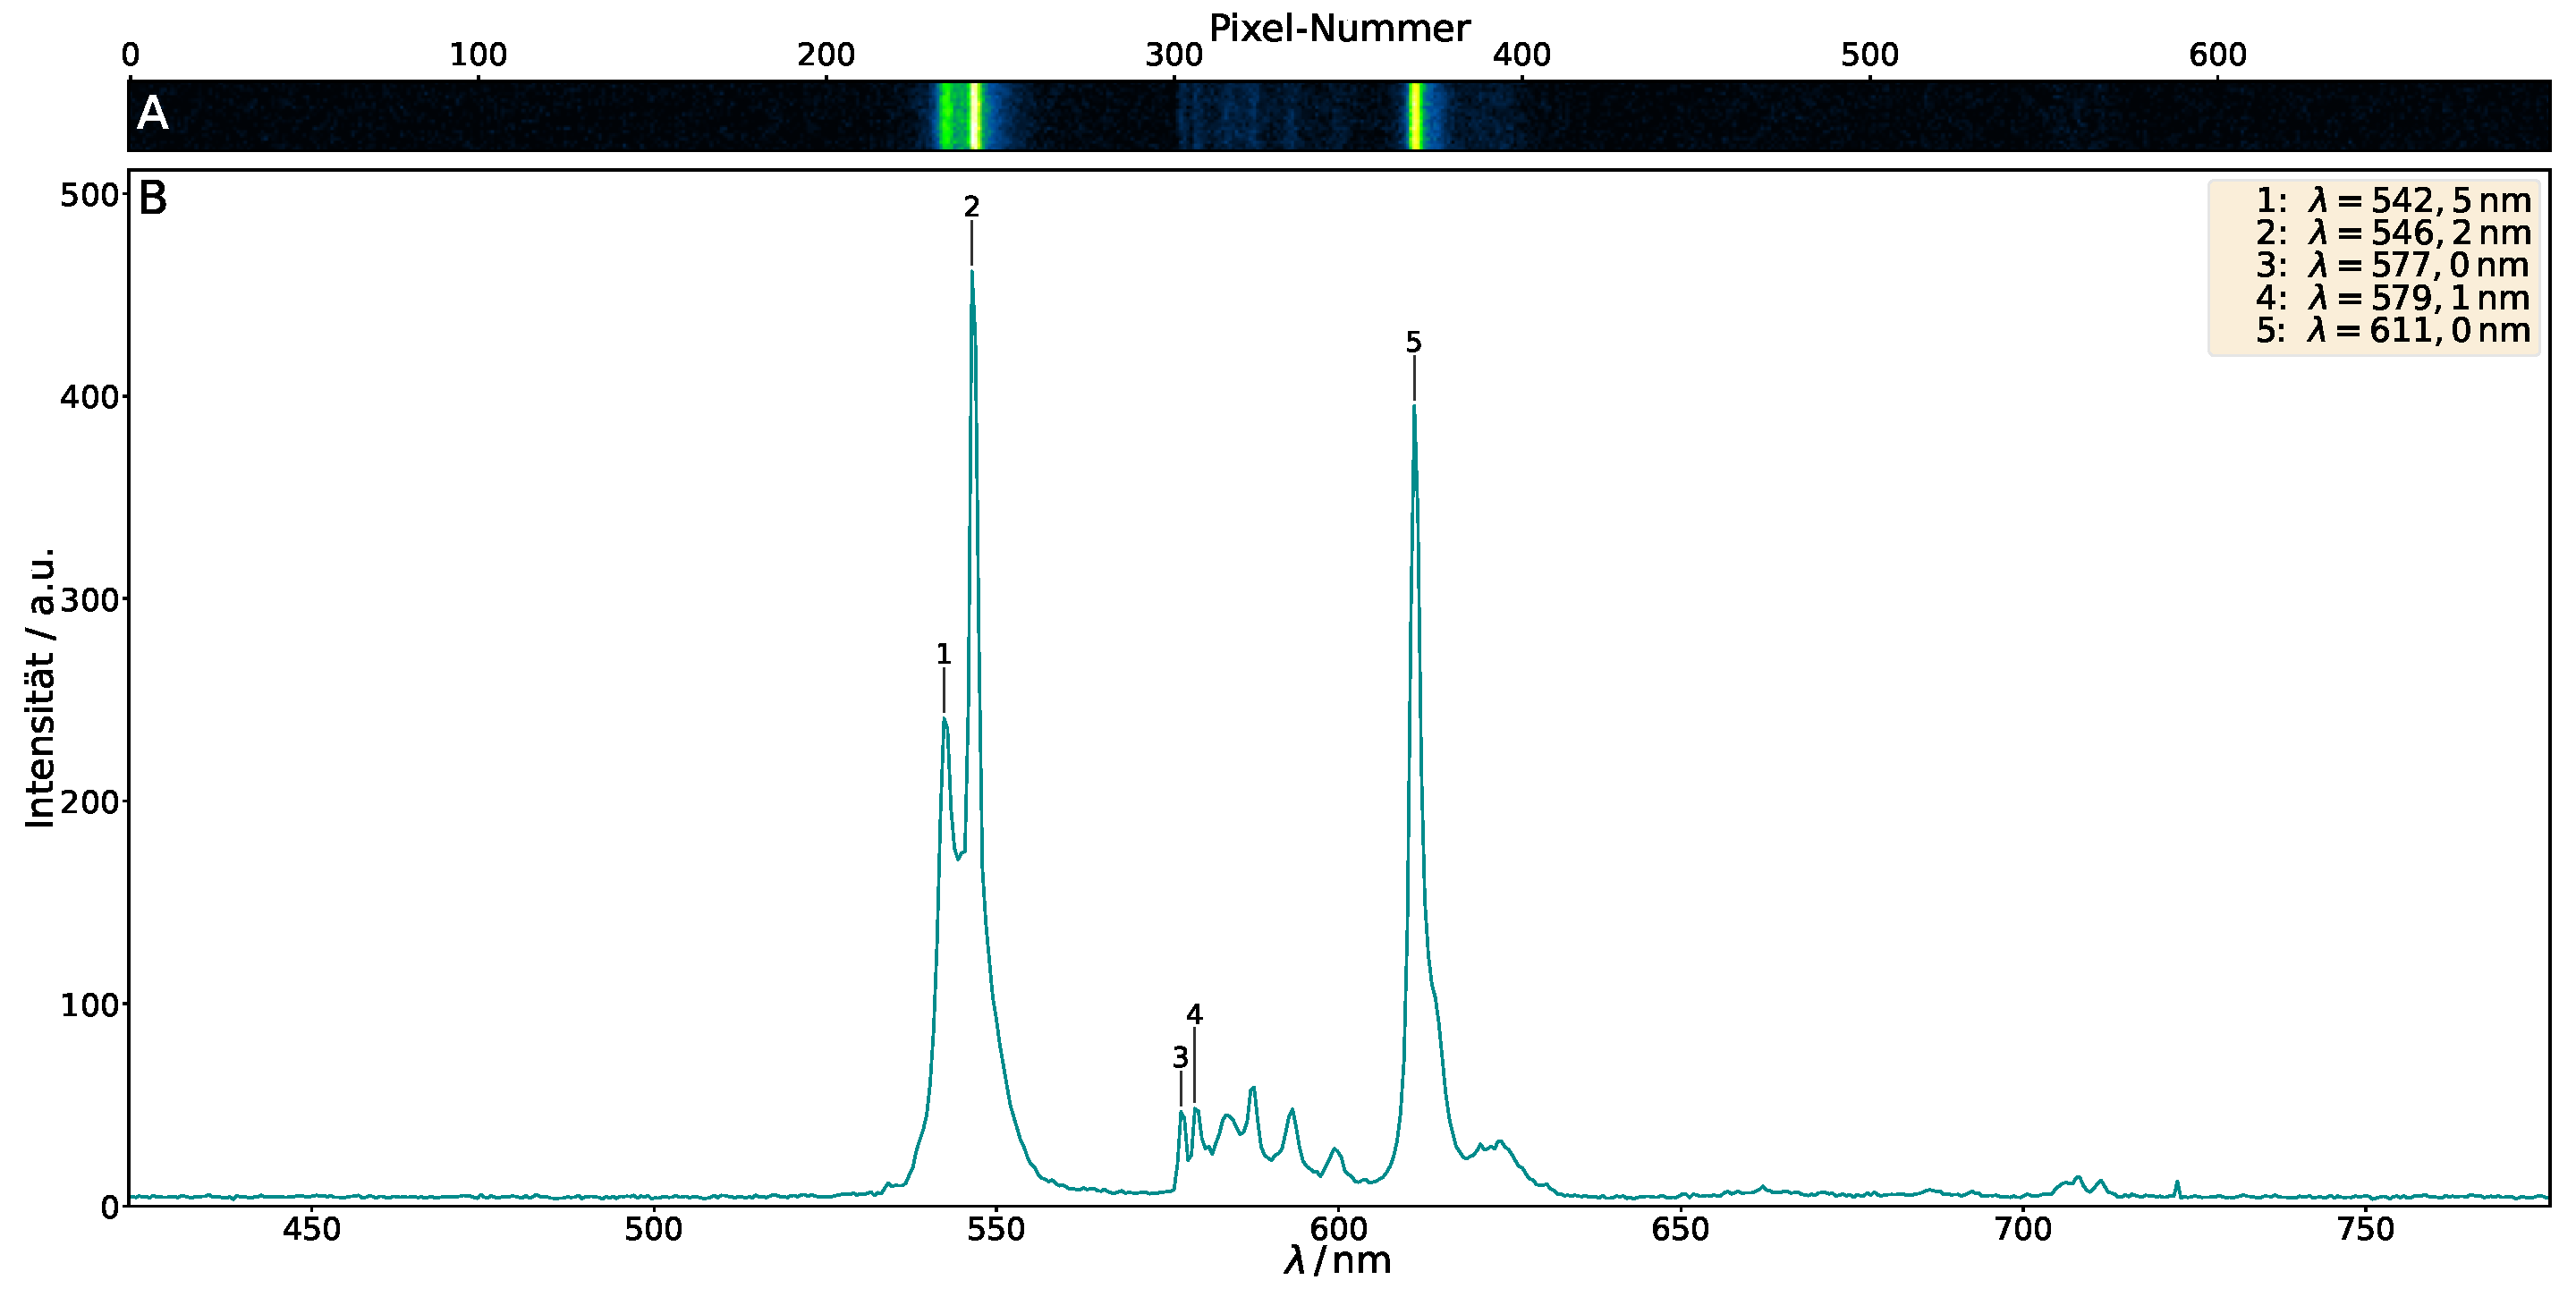
\includegraphics[width=\textwidth]{KalibNeu.pdf}
    \caption{\label{fig:kalib}A) Ein Bildausschnitt des in ImageJ bearbeiteten Lampenspektrums. Das Bild ergibt sich aus 
    Mittelung über acht aufgenommene Bilder und Subtraktion des Hintergrundsignals, sowie Anpassung der optischen Darstellung 
    (Kontrast und Farbschema), wobei Letzteres keinen Einfluss auf die Auswertung hat. Zur Erhaltung der Übersicht wird nur ein 
    kleiner Ausschnitt dargestellt. 
    B) Das hieraus gewonnene Spektrum des Lampenlichts. Zusätzlich sind die identifizierten Peaks, sowie deren zugehörige 
    Wellenlänge eingezeichnet. Die x-Achse beschreibt die kalibrierte Wellenlänge. Die ersten vier Peaks sind 
    Quecksilber-Linien, während der letzte einer Emissionslinie des Leuchtstoffes ($\text{Eu}^{3+}$) entspricht \cite{Anleitung}.}
\end{figure}\FloatBarrier
Trägt man die Pixel-Nummer $N_{\text{pixel}}$ der identifizierten Peaks 
gegen die zugehörige Wellenlänge auf, so kann eine Gerade durch die Messpunkte gelegt 
werden, welche die lineare Transformationsgleichung von der Pixel-Nummer auf 
die Wellenlänge wie folgt beschreibt
\begin{equation}
    \lambda = m\cdot N_{\text{pixel}} + b. 
\end{equation} \newpage
Der zugehörige Graph ist in Abb.~\ref{fig:fit} dargestellt.
\begin{figure}[h!]
    \centering
    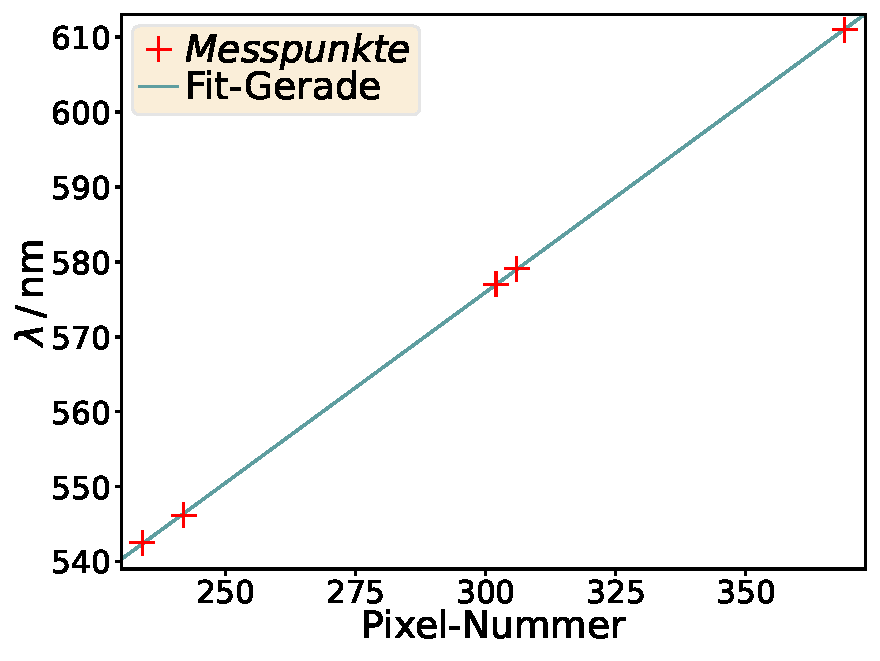
\includegraphics[width=0.6\textwidth]{Fit.pdf}
    \caption{\label{fig:fit}Wellenlänge der identifizierten Linien gegen den zugehörigen 
    Pixelwert. Die zusätzlich eingezeichnete Fit-Gerade beschreibt die lineare Transformation 
    zwischen dem Ort des Pixels und der zugehörigen Wellenlänge des Spektrographen.}
\end{figure}\FloatBarrier
Aus dem in Python errechneten Fit erhalten wir folgende Werte für die Parameter
\begin{alignat}{3}
    m &= 0.508934\,\si{nm}\hspace{2cm}& s_{m} &= 0,001556\,\si{nm}\hspace{2cm} &\Rightarrow \Aboxed{m &= (0,509\pm 0,002)\,\si{nm}} \label{eq:kali}\\
    b &= 423,263674\,\si{nm}\hspace{2cm}& s_{b} &= 0,458771\,\si{nm}\hspace{2cm} &\Rightarrow \Aboxed{b &= (423,3\pm 0,5)\,\si{nm}}.
\end{alignat}
Hieraus lassen sich für alle weiteren Spektren die Pixel-Messwerte in Wellenlängen umrechnen. \\

\subsection{\label{subsec:A2}EMS - Weitfeld-Bild}
Nach der Kalibration wird zunächst die Probe präpariert, 
an welcher die Messungen gemacht werden. Hierbei werden in eine Polystyrol-Matrix (PS) 
Perylenbisimid-Moleküle (PBI) eingebettet, sodass diese immobilisiert und einzeln untersuchbar sind.
Hierzu werden $10\,\si{\mu L}$ einer bereits vorbereiteten $0,1\,\si{nM}$ PBI-Toluol-Lösung in 
$50\,\si{\mu L}$ einer PS-Toluol-Lösung der Konzentration $c=25\,\si{mg/mL}$ pipettiert. 
$25\,\si{\mu L}$ der vermischten Lösung werden auf ein Glasplättchen aufgebracht, welches in 
einem Spincoater dreht. Die Drehfrequenz wird linear auf $\omega=2000\,\si{\frac{1}{\text{min}}}$ 
gesteigert, wobei der Pipetten-Inhalt bei etwa $\omega=1200\,\si{\frac{1}{\text{min}}}$ mit 
einem Schwung auf dem Plättchen entleert wird. Um Verunreinigungen zu vermeiden, werden die benutzten 
Glasflaschen und -plättchen gereinigt und mit einer Flamme kurzzeitig erhitzt. \\
Die Probe wird nach Beendigung des Coating-Prozesses auf dem motorisierten x/y-Verschiebetisch angebracht, 
während auf das Objektiv das Immersionsöl geträufelt wird. Das Deckglas wird mithilfe eines Rädchens 
in den Fokus des Objektivs gefahren, bis das vom Glaskeil (vgl.~Abb.~\ref{fig:aufbau}) reflektierte Licht
einen vorgegebenen Durchmesser erreicht. Der Rückreflex ist dabei auf ein Papierstück mit einem aufgemalten 
Kreis des gewünschten Durchmessers gerichtet, welcher über eine Kamera beobachtet werden kann. 
Während der Justage ist der Shutter geöffnet, die Anregungsleistung jedoch klein gehalten 
($\approx 100\,\si{\mu W}$). \\
Die Weitfeldlinse wird anschließend in den Strahlengang geklappt und der Spektrograph mit weit 
geöffnetem Spalt im Spiegelmodus und Zentralwellenlänge von $0\,\si{nm}$ betrieben. 
Die Anregungsleistung stellen wir auf $490\,\si{\mu W}$ ein, 
wobei Schwankungen von bis zu $10\,\si{\mu W}$ während der Messung beobachtet werden. 
Anhand des Live-Bildes des CCD-Kamera wird die Höhe des Probentischs nochmals fein nachjustiert, 
bis ein scharfes Bild erkennbar ist. Das sich hieraus ergebende Bild, inklusive Hintergrundkorrektur
ist beispielhaft in Abb.~\ref{fig:weitfeldbild} dargestellt. 
\begin{figure}[h!]
    \centering
    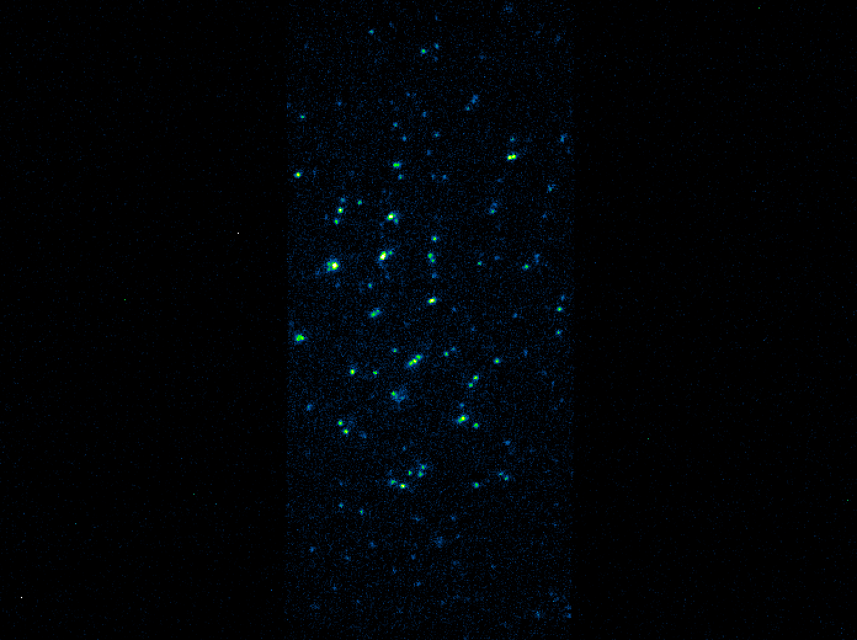
\includegraphics[width=0.5\textwidth]{Weitfeld.png}
    \caption{\label{fig:weitfeldbild}Hintergrundkorregierte Weitfeldaufnahme der hergestellten 
    PBI-Probe in einer PS-Matrix. Die Kamera wird mit 2x2-Binning betrieben. Die schwarzen Balken 
    werden durch die Spalten am Spektrograph erzeugt. Zur besseren optischen Analyse wurde 
    der Kontrast des Bildes, sowie das Farbschema verfeinert.}
\end{figure}\FloatBarrier
Mit dem Verschiebetisch werden nach und nach neue Positionen der Probe angefahren und eine Sequenz 
aus 100 bis 150 Bildern aufgenommen. Nach jeder Messung wird eine Sequenz des Untergrunds bei geschlossenem 
Shutter aufgenommen. Alle Messungen werden ohne Deckenbeleuchtung und mit Lichtschutz um den Messaufbau 
durchgeführt, um das Hintergrundsignal so klein wie möglich zu halten. Nachdem der gemittelte Untergrund 
von jedem Bild der Sequenz abgezogen wurde, kann an einem beliebigen Pixel-Pfad in x- und y-Richtung der 
zeitliche Verlauf der Pixelintensität (des Grauwertes) dargestellt werden. 
Dies erlaubt die zeitaufgelöste Messung der Fluoreszenz einzelner Moleküle, 
wodurch Effekte wie Blinken und Photobleichen beobachtet werden können. 
Beispielhafte Beobachtungen solcher Prozesse sind im folgenden Abschnitt präsentiert. \\
Beschreibt man die Breite des Bildes mit einer $x$-Koordinate und die Höhe mit der $y$-Koordinate, so kann 
bei der bearbeiteten Bildsequenz an einer beliebigen Stelle $x$ der Intensitätsverlauf in $y$-Richtung
als Funktion der Zeit dargestellt werden (\textit{Orthogonal Views} in ImageJ). 
Abb.~\ref{fig:beispielBlink} A zeigt den entstehenden Bildausschnitt. Mithilfe der \textit{Plot Profile}
Funktion lässt sich die Pixelintensität als Funktion der Zeit darstellen, was für drei Beispiel-Moleküle 
in Abb.~\ref{fig:beispielBlink} B-D gemacht wird. 
\begin{figure}[h!]
    \centering
    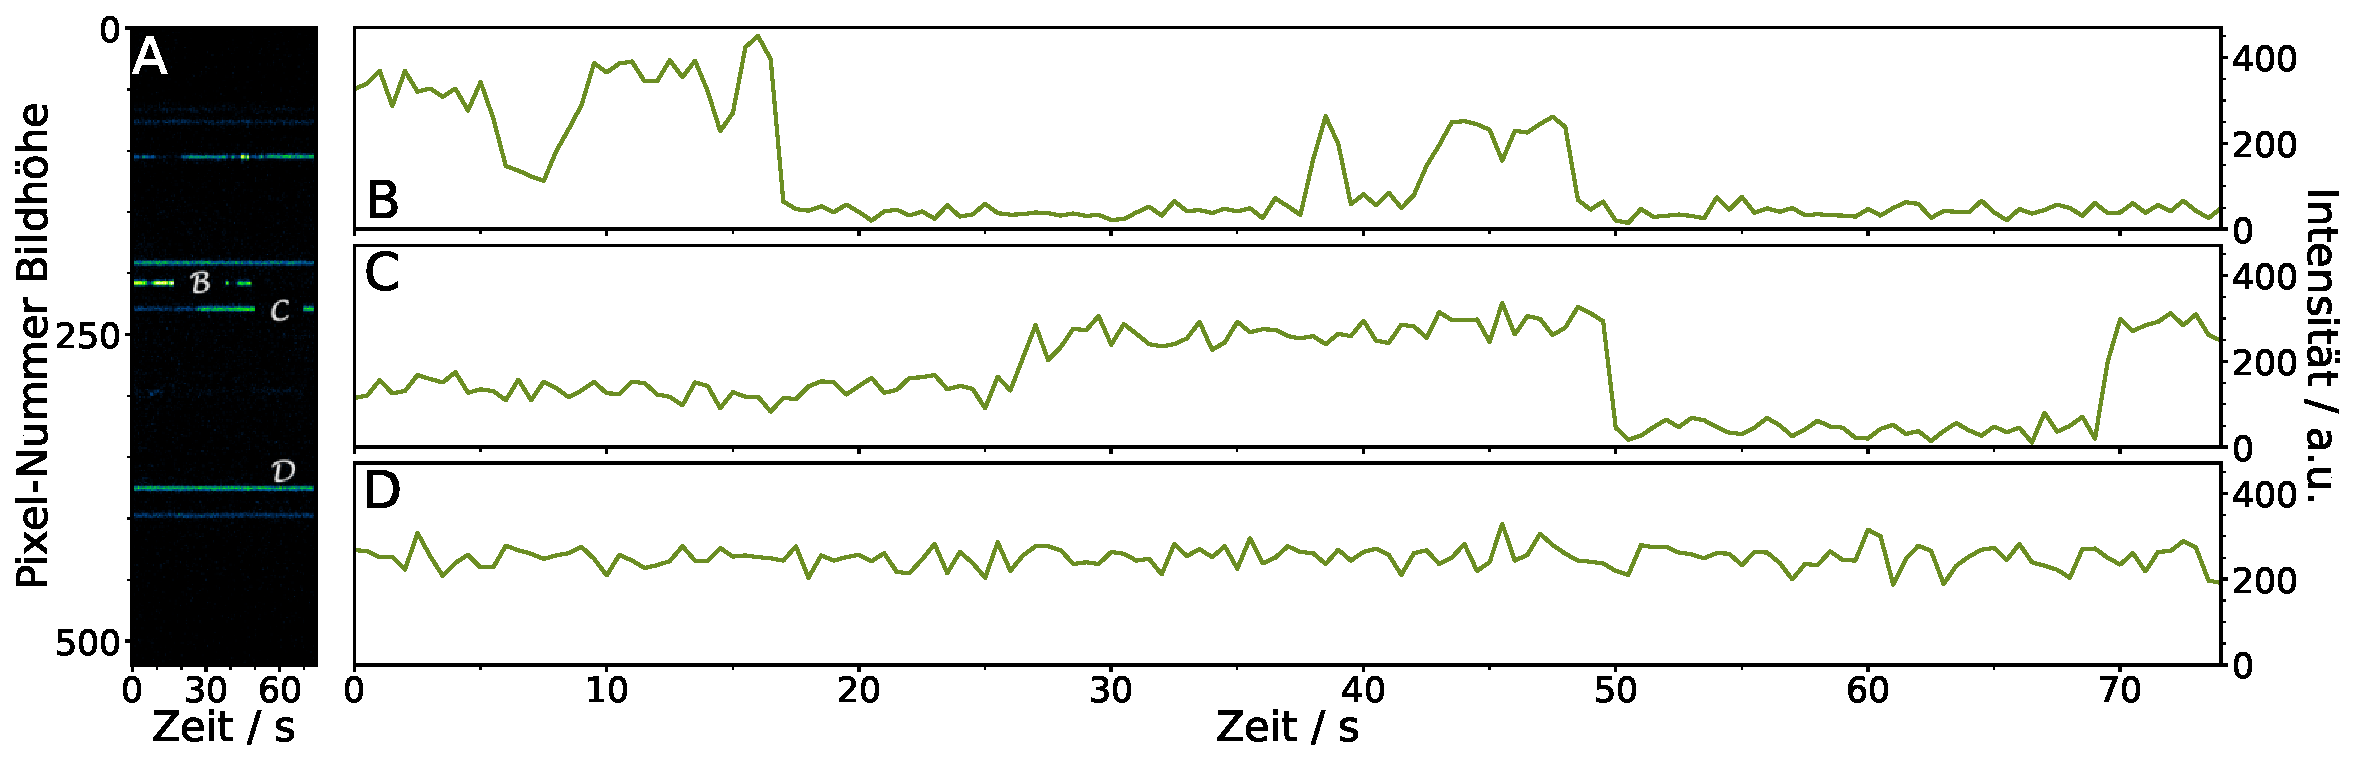
\includegraphics[width=\textwidth]{BlinkBsp.pdf}
    \caption{\label{fig:beispielBlink}A) \textit{Orthogonal Views}-Bildausschnitt aus ImageJ einer 
    beispielhaften Bildsequenz aus 150 Bildern mit einer Belichtungszeit von $500\,\si{ms}$. Die x-Achse beschreibt den 
    zeitlichen Verlauf, die y-Achse zeigt die Bildhöhe an einer beliebig gewählten Stelle $x$ der Bildsequenz. Die geschweiften 
    Buchstaben sind mit den nebenstehenden Achsen verknüpft. B-D) Die sich aus der \textit{Plot Profile}-Funktion ergebenden 
    zeitlichen Intensitätswerte der betrachteten Moleküle. Zur Analyse wird ein kleiner Bereich aus wenigen Pixeln (Höhe) verwendet.}
\end{figure}\FloatBarrier
Das in ImageJ bearbeitete Bild zeigt die Pixelintensität (Helligkeit) als Funktion 
der Zeit an. Ein leuchtender horizontaler Strich ist daher mit 
einem fluoreszierendem Molekül zu identifizieren, welches über den 
gesamten Beobachtungszeitraum Photonen emittiert (D). 
Da ein solches Signal auch durch Verunreinigungen oder durch mehrere 
Fluorophore auf einem Fleck entstehen kann, ist es sinnvoll, das Signal 
als Funktion der Zeit zu betrachten. 
Dadurch können Effekte wie Photobleaching der Moleküle (möglicherweise B) 
oder Blinking (C) erkannt werden, woraus man folgern kann, 
dass tatsächlich ein fluoreszierendes Molekül betrachtet wird. \\
Das Photobleaching ist ein irreversibler Prozess, der durch Licht-induzierte 
chemische Reaktionen verursacht wird und das Fluorophor in ein Molekül mit 
deutlich verringerten Emissionswahrscheinlichkeiten umwandelt, 
wodurch eine Limitierung der Beobachtungszeit des Fluorophors entsteht.
Nach dieser Umwandlung ist das Fluoreszenzsignal nicht mehr vorhanden bzw.~nicht vom 
Untergrund unterscheidbar.
Blinking hingegen ist gekennzeichnet durch eine reversible Abnahme 
oder das Verschwinden der Emission einzelner Moleküle im Mikro- bis Sekundenbereich.
Ursachen hierfür sind z.B.~die Besetzung angeregter nicht emittierender Triplettzustände,
Prozesse wie molekulare Rotation, spektrale Verschiebung aufgrund lokaler 
Wechselwirkungen oder konformationelle Änderungen (Fotoisomere).
Die Lebensdauer von Tripletzuständen hängt von der Konzentration von 
molekularem Sauerstoffkonzentration ab und liegt im Mikro- bis Millisekundenbereich.
Fotoisomere dagegen können Ihre Form bis zu mehrere Sekunden lang halten und reversibel 
verändern, was zu einer langanhaltenden Änderung im Fluoreszenzsignal führt, 
die wir bei unseren Messungen beobachten können \cite{fluo}. \\
In Abb.~\ref{fig:beispielBlink} ist das Blinking in Fall B und C 
zu erkennen. Teilweise sinkt die Intensität bis zum Untergrundsignal 
oder zu einem schwächeren Zwischenzustand (ersten $20\,\si{s}$ bei C). 
Der nicht emittierende Zwischenzustand kann viele Sekunden existieren, 
sodass im gemessenen Zeitintervall nicht eindeutig identifiziert werden kann, 
ob es sich um ein blinkendes Molekül oder ein ausgeblichenes Molekül 
handelt. Aus der Beobachtung vieler Moleküle kann jedoch abgeschätzt werden, 
dass die Blinkzeit meist unterhalb von $35\,\si{s}$ liegt.
In Abb.~\ref{fig:blinken} ist für drei intensitätsstarke 
exemplarische Moleküle das Blinken gezeigt, während 
in Abb.~\ref{fig:sterben} Beispiele für das Photobleaching
dargestellt sind.
\begin{figure}[h!]
    \centering
    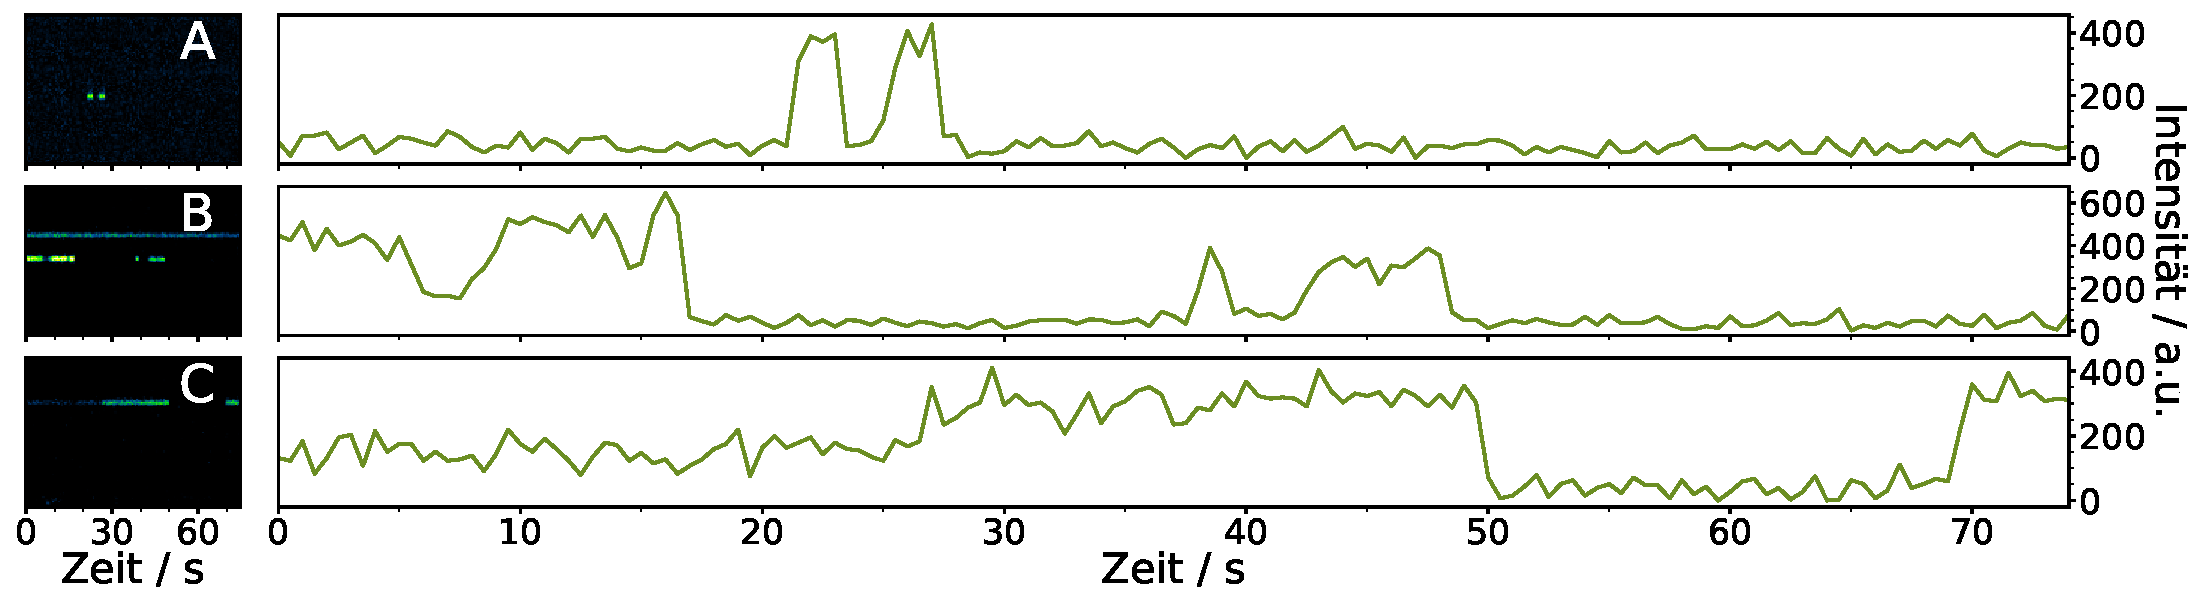
\includegraphics[width=\textwidth]{Blinken.pdf}
    \caption{\label{fig:blinken}Das Intensitätssignal eines Pixelbereichs als Funktion
    der Zeit für drei ausgewählte Moleküle die ein Blinkverhalten zeigen. Auf der linken 
    Seite ist jeweils ein Bildausschnitt des in ImageJ bearbeiteten Bildes zu erkennen. 
    Die rechte Seite ergibt sich aus der \textit{Plot Profile} Funktion um einem engen 
    Pixelbereich, der das betrachtete Molekül enthält. Das Signal errechnet sich aus einer 
    Bildsequenz mit 150 Bildern mit einer Belichtungszeit von $500\,\si{ms}$ und der 
    entsprechenden Hintergrundkorrektur.}
\end{figure}\FloatBarrier
Molekül A zeigt für jeweils zwei Zeiträume von etwa $5\,\si{s}$ Fluoreszenz und scheint danach 
auszubleichen. Molekül B verändert mit der Zeit zusätzlich die Intensität, nachdem 
es sich für ca.~$20\,\si{s}$ in einem nicht emittierenden Zustand befunden hat.
Auch im Fall C ist gegen Ende der Beobachtungszeit ein Blinken zu erkennen, wobei zwischen 
den Fluoreszenzsignalen das detektierte Signal auf das Untergrundlevel abfällt.  
\begin{figure}[h!]
    \centering
    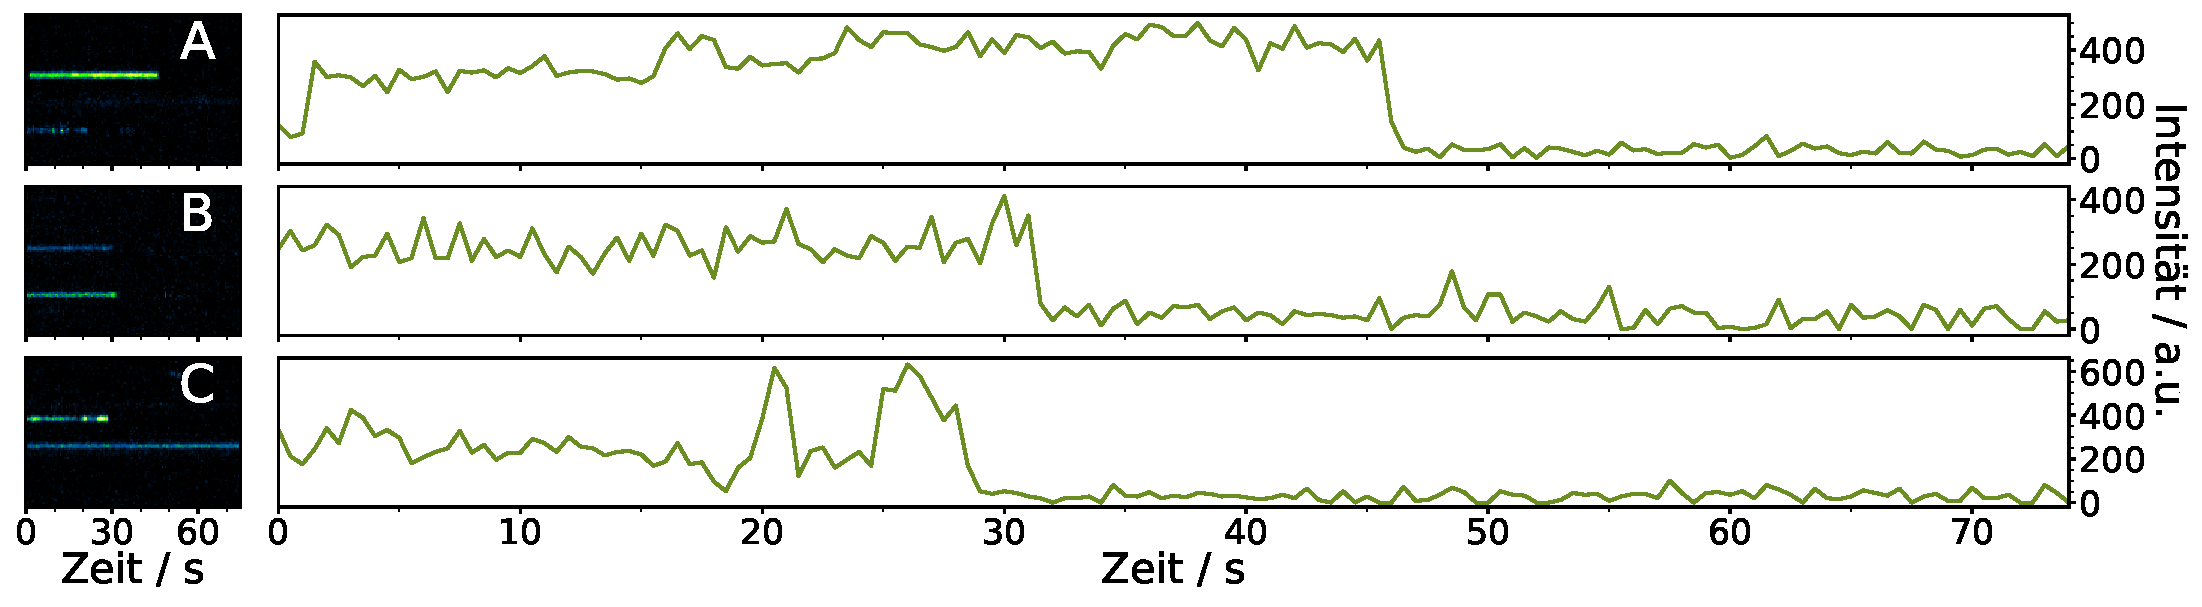
\includegraphics[width=\textwidth]{Sterben.pdf}
    \caption{\label{fig:sterben}Das Intensitätssignal eines Pixelbereichs als Funktion
    der Zeit für drei ausbleichende Moleküle. Berechnungsschritte und Darstellung sind 
    analog zu vorheriger Abbildung (Abb.~\ref{fig:blinken}) gewählt.}
\end{figure}\FloatBarrier
Für alle Moleküle A,B,C ist nach einer gewissen Zeit ein Abklingen des Fluoreszenzsignals 
bis zum Untergrundsignal erkennbar. Im betrachteten Messintervall erstarkt das Signal 
nicht mehr, woraus wir schließen, dass die Moleküle ausgeblichen sind. 
Im Gegensatz zu Molekül C, scheinen die ersten beiden Moleküle mit konstanter Intensität
zu fluoreszieren. Eine tiefgehende Erklärung dieser Effekte wird in diesem Praktikumsbericht 
nicht geliefert, kann jedoch für andere Fluorophore in Ref.~\cite{fluo} nachgelesen werden.\\
Insgesamt erkennen wir in verschiedenen Bildsequenzen viele Fälle mit 
Photobleaching und Blinking, woraus wir schließen, dass die 
Probenpräparation erfolgreich verlaufen ist und wir somit tatsächlich 
das Fluoreszenzsignal einzelner Moleküle messen. Zudem wird die korrekte 
Justage des Versuchsaufbaus bestätigt, womit wir den ersten Versuchsteil 
erfolgreich abschließen. \\

\subsection{\label{subsec:A3}EMS - Polarisation der Fluoreszenz}
Zur Untersuchung der Polarisationsabhängigkeit der Fluoreszenz wird der rotierende Polarisator in den 
Strahlengang geklappt. Dieser rotiert mit einer Frequenz von $f\approx 0,15\,\si{s^{-1}}$ und 
polarisiert das zirkulare Anregungslicht linear in Richtung seiner aktuellen Stellung. 
Mit den gleichen Einstellungen wie in vorherigem Abschnitt und einer Anregungsleistung von $325\pm5\,\si{\mu W}$ werden 
Sequenzen aus 150 Bilder aufgenommen, 
die mit einem direkt hiernach aufgenommenen Hintergrund korrigiert werden. \\
In Abb.~\ref{fig:polari} stellen wir das Fluoreszenzsignal einiger beispielhafter Moleküle als Funktion der 
Detektionszeit dar. Die Bildverarbeitung und Datengewinnung sind hierbei analog zu vorherigem Abschnitt.
\begin{figure}[h!]
    \centering
    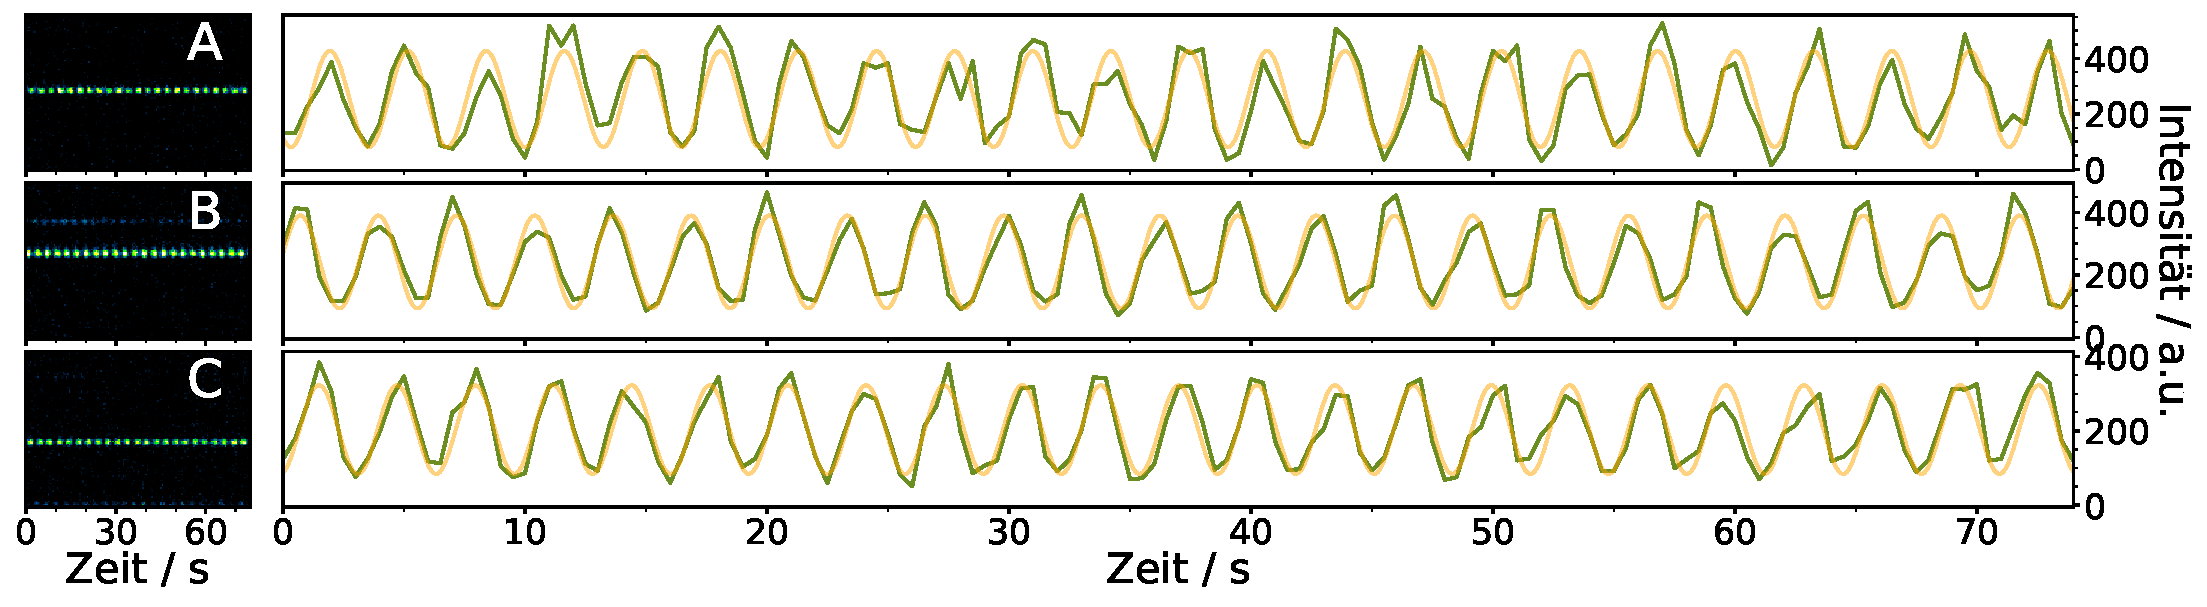
\includegraphics[width=\textwidth]{Polarisation.pdf}
    \caption{\label{fig:polari}Das Intensitätssignal eines Pixelbereichs als Funktion
    der Zeit für drei ausgewählte Moleküle. 
    Während der Messung wird das Licht mit einem rotierendem
    Polarisator linear polarisiert. Es wird jeweils eine Bildsequenz aus 150 Bildern mit einer Belichtungszeit von 
    $500\,\si{ms}$ aufgenommen, die hiernach vom Untergrundsignal bereinigt wird. Der Bildausschnitt links zeigt jeweils 
    ein Bildausschnitt aus ImageJ des betrachteten Moleküls. Das Intensitätssignal (grün) auf der rechten Seite ergibt sich 
    hieraus mithilfe der \textit{Plot Profile} Funktion. An das Signal wird ein Cosinus gefittet (orange), dessen 
    jeweilige Parameter im Haupttext diskutiert sind.}
\end{figure}\FloatBarrier
Die Stärke der Absorption und Emission von Licht wird durch die Orientierung der Dipolmomente der Moleküle während des 
Übergangs bestimmt. In vielen Fällen sind die Dipolmomente der Moleküle entlang einer bestimmten Achse ausgerichtet, 
was dazu führt, dass die emittierte Fluoreszenz linear polarisiert ist, wobei ihre Ausrichtung 
von der Orientierung der Moleküle abhängt \cite{Prinzip}. Zudem wird Licht nur entlang einer Achse absorbiert, 
wodurch man eine Polarisationsabhängigkeit im Fluoreszenzsignal erkennen kann. \\
Für alle drei Moleküle und sehr viele weitere, die wir beobachten konnten, wird die 
Abhängigkeit des Fluoreszenzsignals von der Lichtpolarisation bestätigt. 
Mit einer bestimmten Frequenz $f$ erstarkt und erlischt das Signal in allen Fällen. 
Die Intensität fällt dabei sehr stark ab, erreicht bei unseren Beobachtungen jedoch 
nicht immer den Untergrund, was an der langen Belichtungszeit liegen könnte. 
Die Messungen entsprechen dennoch den Erwartungen. \\
Wird ein Cosinus an die betrachteten Signale gefittet, so lässt sich hieraus
die Rotationsfrequenz des Polarisators und die Phasenlage zueinander bestimmen. 
Aus der gegenseitigen Phasenlage kann die Orientierung der Moleküle zueinander bestimmt
werden, da diese immobilisiert sind. 
Folgende Funktion wählen wir als gefittete Kurve
\begin{equation}
    a\cdot\cos\left(2\pi(f\cdot t-\delta)\right) + b.
\end{equation}
Aus den drei Signalen ergeben sich folgende Werte inklusive der zugehörigen Fehler
\begin{alignat}{5}
    a &= (173 \pm 7)\hspace{1cm}& f &= (0,3099 \pm 0,0003)\,\si{s^{-1}}\hspace{1cm}& \delta &= (0,601 \pm 0,013)\hspace{1cm}& b &= (253 \pm 5) \\
    a &= (149 \pm 4)\hspace{1cm}& f &= (0,3096 \pm 0,0002)\,\si{s^{-1}}\hspace{1cm}& \delta &= (0,221 \pm 0,009)\hspace{1cm}& b &= (241 \pm 3) \\
    a &= (120 \pm 4)\hspace{1cm}& f &= (0,3096 \pm 0,0002)\,\si{s^{-1}}\hspace{1cm}& \delta &= (0,459 \pm 0,010)\hspace{1cm}& b &= (203 \pm 3).
\end{alignat}
Insgesamt erhalten wir hieraus für den Fitparameter $f$
\begin{equation}
    \fbox{$f = (0,30970 \pm 0,00015)\,\si{s^{-1}}$}.
\end{equation}
Die Rotationsfrequenz des Polarisators $f_{\text{P}}$ ist die Hälfte des Parameters $f$, 
da die richtige lineare Polarisation bei einer kompletten Umdrehung zweimal erreicht wird. 
Damit liegt der Wert im Bereich der in der Anleitung angegebenen Rotationsfrequenz von 
$f_{\text{P}}\approx0,15\,\si{s^{-1}}$. \\
Die Phasenlage $\delta$ ist für die betrachteten Moleküle sehr unterschiedlich und zeigt daher, 
dass die Moleküle anisotrop angeordnet sind. \\ 
Zusammengefasst kann der zweite Versuchsteil als gelungen verbucht werden. Die Ergebnisse sind eindrucksvoll 
und schön und sie entsprechen den Erwartungen. \\

\subsection{\label{subsec:A4}EMS - Spektren}
Abschließend wollen wir die Spektren einzelner Moleküle betrachten und mit dem Ensemblespektrum vergleichen. 
Hierzu wird die Weitfeldlinse entfernt und der Spektrograph im Gittermodus betrieben, wobei die 
Zentralwellenlänge analog zur Kalibration auf $\lambda=600\,\si{nm}$ eingestellt wird. Die Anregungsleistung ist 
auf $205\pm5\,\si{\mu W}$ reduziert und die Spaltbreite geregelt, dass die Spektren scharf erkennbar sind, 
was bei einer Breite von $0,3\,\si{mm}$ der Fall ist. \\
Mit diesen Einstellungen suchen wir mithilfe des Verschiebetischs insgesamt 30 gut erkennbare Einzelmoleküle, 
deren Signal wir für mindestens $15\,\si{s}$ (30 Bilder bei einer Belichtungszeit von $500\,\si{ms}$) aufnehmen. 
Hiernach wird bei geschlossenem Shutter das Untergrundsignal für einige Sekunden aufgenommen. \\
Die jeweiligen Aufnahmesequenzen werden gemittelt, um das Signal-Rausch-Verhältnis zu verbessern und hiernach vom 
gemittelten Untergrund subtrahiert. Das entstehende Bild wird mit Kontrast- und Farbschema-Regelung aufgehübscht 
und abgespeichert. Mithilfe der \textit{Plot Profile} Funktion lässt sich das Spektrum analysieren.
Zur Bestimmung der Übergangswellenlängen wird ein Pseudo-Voigt-Profil an das errechnete und normierte Spektrum gefittet, 
da die optische Übereinstimmung besser als bei einem Gauß-Fit ist. 
Für die angefittete Funktion gilt
\begin{align}
    F(\lambda) &= \sum_{i=1}^{3}\,a_{i}\cdot V_{i}(\lambda) + b_{i} \\
    V_{i}(\lambda) &= \eta \cdot L_{i}(\lambda) + (1-\eta )\cdot G_{i}(\lambda),\hspace{0.5cm}\eta\,\in\,(0,\,1) \\
    G_{i}(\lambda) &= e^{-\ln(2)\cdot\left(\frac{\lambda - \mu_{i}}{\sigma_{i}}\right)^{2}} \\
    L_{i}(\lambda) &= \left[1+\left(\frac{\lambda - \mu_{i}}{\sigma_{i}}\right)^{2}\right]^{-1}.
\end{align}
Die Parameter werden in Bereiche eingegrenzt, sodass der in Python durchgeführte Fit-Algorithmus sinnvolle 
Ergebnisse liefert. Für die weitere Auswertung interessiert uns der Parameter $\mu_{i}$, welcher die Wellenlänge des 
Übergangs angibt. Eine Auflistung der Werte und der zugehörigen Fehler ist in Tab.~\ref{tab:lamda} dargestellt. 
Der Fehler ergibt sich rein aus dem im Fit-Algorithmus errechneten, da er den 
Kalibrationsfehler aus Gl.~\ref{eq:kali} weit übertrifft. Gerade die Wellenlängenbestimmung für den 
Übergang $0^{*}\rightarrow 2$ ist mit großem Fehler behaftet, da das Signal des Übergangs oft kaum vom Untergrundsignal 
unterscheidbar ist. 
\begin{table}[h!]
    \centering
    \caption{\label{tab:lamda}Mit dem Fit-Algorithmus berechnete Werte von $\mu_{i} = \lambda_{i}$. Für alle 30 Einzelmolekül-Spektren (Nummer),
    sind drei Wellenlängen der Fluoreszenzübergänge $0^{*}\rightarrow0\,(\lambda_{1})$, $0^{*}\rightarrow1\,(\lambda_{2})$ und 
    $0^{*}\rightarrow2\,(\lambda_{3})$ aufgelistet. Der zugehörige Fehler ergibt sich auf dem Fit-Algorithmus, wobei 
    der Kalibrationsfehler aus Abschnitt \ref{subsec:A1} vernachlässigt werden kann.}
      \begin{tabular}{c|c|c|c|c|c|c}
      \rowcolor[rgb]{ .663,  .816,  .557} Nummer & $\lambda_{1}\,/\,\si{nm}$ & $\lambda_{2}\,/\,\si{nm}$ & $\lambda_{3}\,/\,\si{nm}$ &
      $s_{\lambda_{1}}\,/\,\si{nm}$ & $s_{\lambda_{2}}\,/\,\si{nm}$ & $s_{\lambda_{3}}\,/\,\si{nm}$ \\
      \hline \hline
      1     & 538,0 & 576,6 & 624,9 & 4,1   & 5,5   & 25,0 \\
      2     & 546,1 & 584,4 & 640,5 & 2,3   & 6,0   & 7,1 \\
      3     & 534,6 & 566,0 & 616,8 & 4,1   & 11,6  & 24,7 \\
      4     & 534,8 & 570,0 & 620,7 & 5,1   & 9,7   & 26,4 \\
      5     & 536,9 & 573,5 & 624,6 & 4,0   & 7,5   & 9,4 \\
      6     & 537,6 & 575,7 & 615,4 & 4,9   & 5,9   & 13,7 \\
      7     & 535,4 & 572,4 & 620,9 & 4,5   & 6,5   & 14,2 \\
      8     & 537,6 & 574,9 & 626,8 & 4,2   & 6,4   & 15,3 \\
      9     & 536,5 & 574,7 & 620,1 & 3,8   & 5,3   & 14,2 \\
      10    & 538,6 & 577,5 & 621,8 & 3,6   & 4,7   & 10,8 \\
      11    & 537,6 & 577,1 & 622,7 & 3,4   & 3,9   & 10,6 \\
      12    & 536,4 & 571,8 & 620,0 & 4,9   & 8,7   & 20,0 \\
      13    & 538,2 & 576,7 & 624,0 & 3,1   & 4,0   & 18,0 \\
      14    & 535,6 & 573,3 & 622,4 & 3,7   & 5,6   & 18,3 \\
      15    & 542,5 & 580,2 & 630,0 & 2,8   & 7,4   & 12,2 \\
      16    & 540,8 & 581,4 & 627,9 & 3,4   & 4,0   & 12,1 \\
      17    & 538,9 & 576,0 & 622,8 & 4,0   & 6,6   & 16,0 \\
      18    & 538,5 & 570,6 & 625,5 & 3,4   & 12,2  & 13,3 \\
      19    & 540,6 & 580,5 & 626,1 & 4,2   & 3,7   & 6,4 \\
      20    & 536,1 & 571,7 & 619,3 & 3,8   & 7,5   & 15,9 \\
      21    & 542,5 & 582,8 & 627,0 & 3,0   & 3,6   & 9,4 \\
      22    & 541,5 & 580,3 & 623,7 & 4,7   & 5,2   & 13,7 \\
      23    & 539,6 & 579,3 & 620,6 & 3,5   & 4,2   & 6,7 \\
      24    & 536,5 & 574,4 & 624,3 & 4,6   & 4,9   & 13,3 \\
      25    & 537,2 & 577,0 & 623,2 & 3,7   & 4,1   & 5,7 \\
      26    & 540,3 & 579,2 & 626,8 & 2,9   & 3,9   & 15,6 \\
      27    & 535,2 & 564,0 & 607,9 & 5,4   & 6,7   & 27,6 \\
      28    & 538,6 & 578,2 & 626,8 & 3,4   & 4,4   & 9,6 \\
      29    & 543,4 & 580,8 & 622,4 & 3,3   & 7,9   & 3,1 \\
      30    & 536,1 & 571,7 & 619,3 & 3,8   & 7,5   & 15,9 \\
      \end{tabular}   
\end{table} \FloatBarrier
Mit Tab.~\ref{tab:lamda} erhalten wir für die Wellenlängen der Fluoreszenzübergänge
\begin{equation}
    \fbox{$0^{*}\rightarrow0:\,\,\lambda_{1} = (538,4 \pm 0,7)\,\si{nm}$}\hspace{1cm}
    \fbox{$0^{*}\rightarrow1:\,\,\lambda_{2} = (575,7 \pm 1,2)\,\si{nm}$}\hspace{1cm}
    \fbox{$0^{*}\rightarrow2:\,\,\lambda_{3} = (623 \pm 3)\,\si{nm}$}.
\end{equation}
Die errechneten Wellenlängen sind im Bereich der Erwartung aus Ref.~\cite{Anleitung}.
Hieraus können die Energiedifferenzen der elektronischen Zustände wie folgt berechnet werden
\begin{align}
    E &= \frac{h\,c}{n\,\lambda} \\
    \xrightarrow{n=n_{\text{Luft}}\approx 1} \frac{\Delta{E}_{ij}}{hc} &= \left(\lambda_{i}^{-1} - \lambda_{j}^{-1}\right) \\
    s_{\frac{\Delta{E}_{ij}}{hc}} &= \sqrt{\left(\frac{s_{\lambda{i}}}{\lambda_{i}^{2}}\right)^{2} + \left(\frac{s_{\lambda{j}}}{\lambda_{j}^{2}}\right)^{2}}.
\end{align}
Insgesamt erhalten wir
\begin{equation}
    \fbox{$\frac{\Delta{E}_{01}}{hc} = (1204\pm43)\,\si{cm^{-1}}$}\hspace{2cm}\fbox{$\frac{\Delta{E}_{12}}{hc} = (1321\pm90)\,\si{cm^{-1}}$}.
\end{equation}
Abschließend werden in Abb.~\ref{fig:spektren} zum Zweck der besseren Visualisierung vier ausgewählte Molekülspektren dargestellt.
Da die Spektren auf ihren jeweiligen Maximal-Intensitätswert normiert sind, wird dieser pro Spektrum angegeben, um Informationsverluste 
zu vermeiden. Alle Spektren werden mit der \textit{Plot Profile} Funktion in ImageJ errechnet, wobei jeweils drei Pixel Höhe 
als Berechnungsbereich ausgewählt sind, um Vergleichbarkeit zu wahren. Die maximalen Grauwerte der Pixel aller Molekülspektren 
befinden sich hierbei in einem Bereich von 115 bis 312 Einheiten.
\begin{figure}[h!]
    \centering
    \subfloat[Nummer 13 - $I_{\text{max}}$/a.u.$=229$]{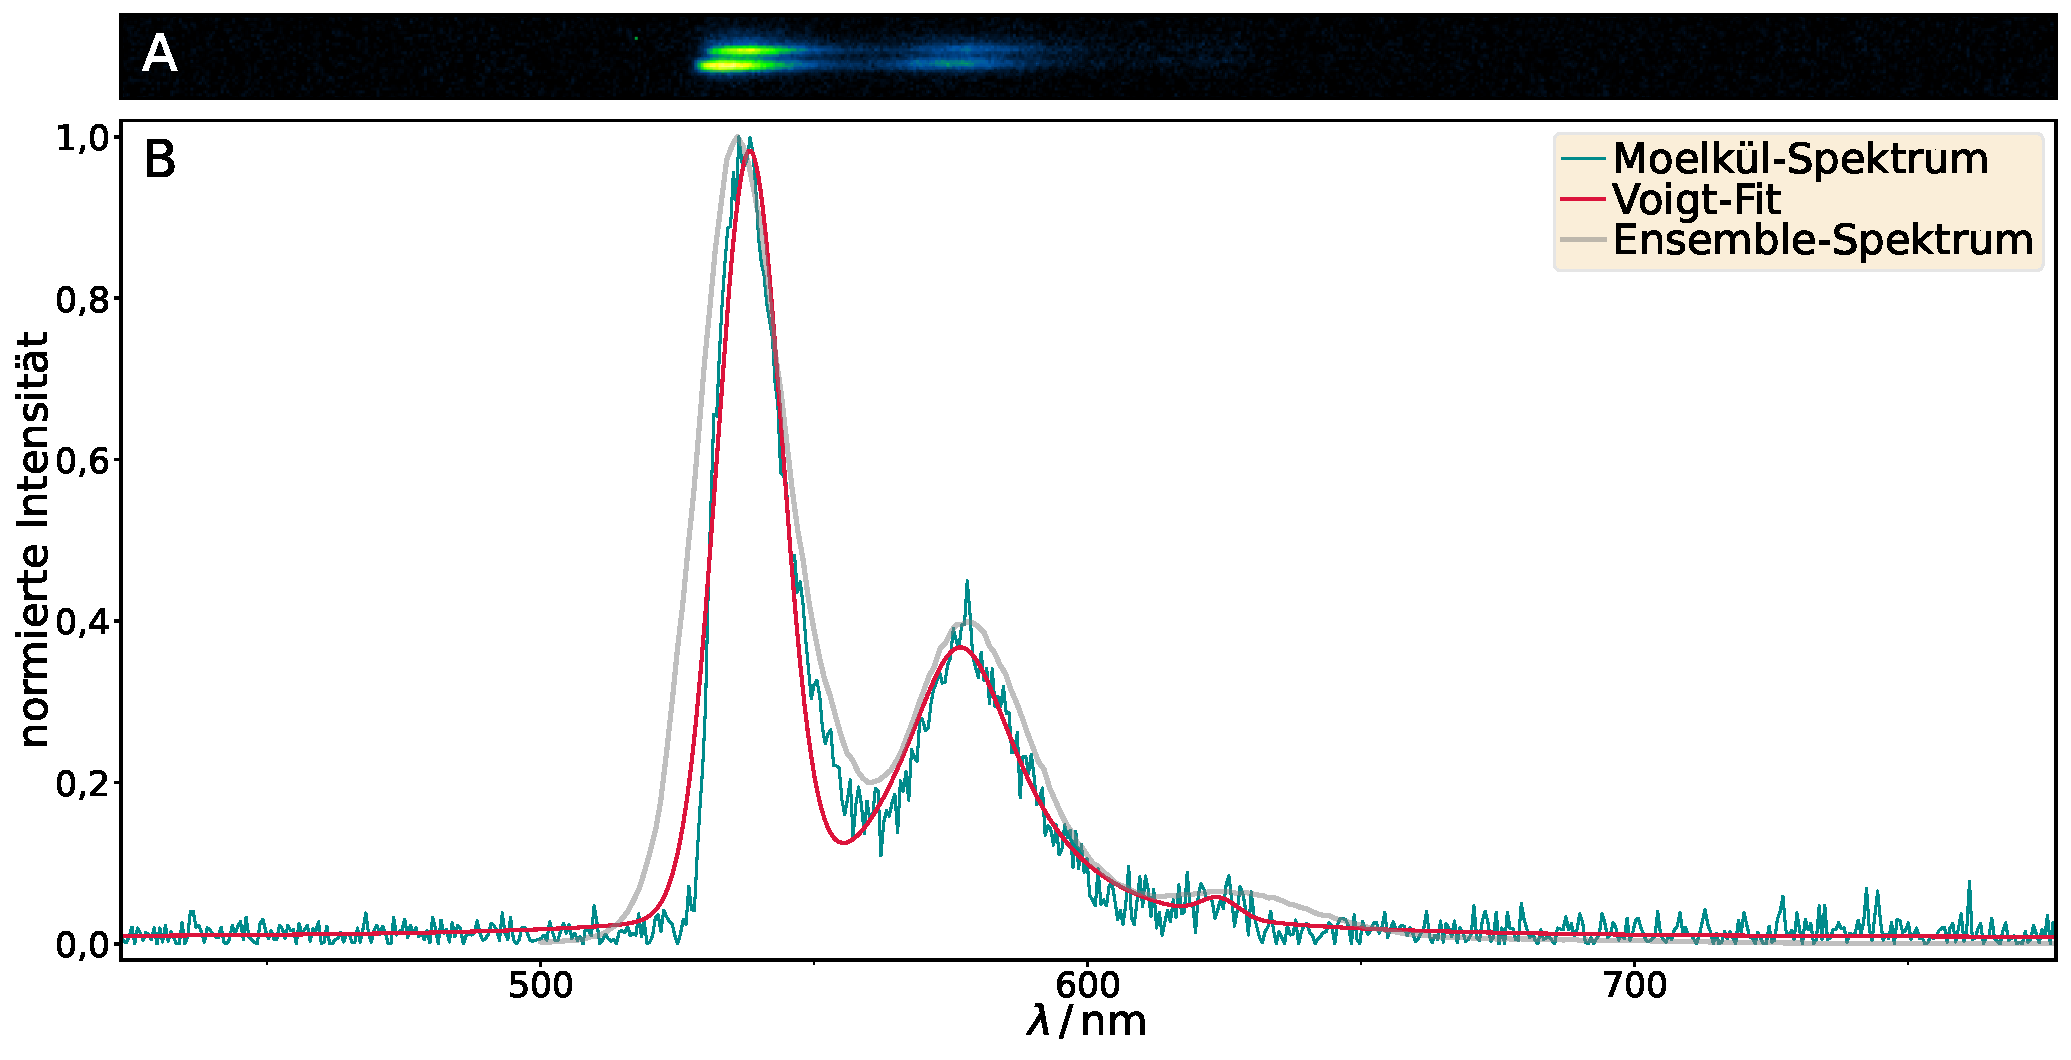
\includegraphics[width=0.49\textwidth]{Spektren/SP13-229.pdf}}
    \subfloat[Nummer 10 - $I_{\text{max}}$/a.u.$=312$]{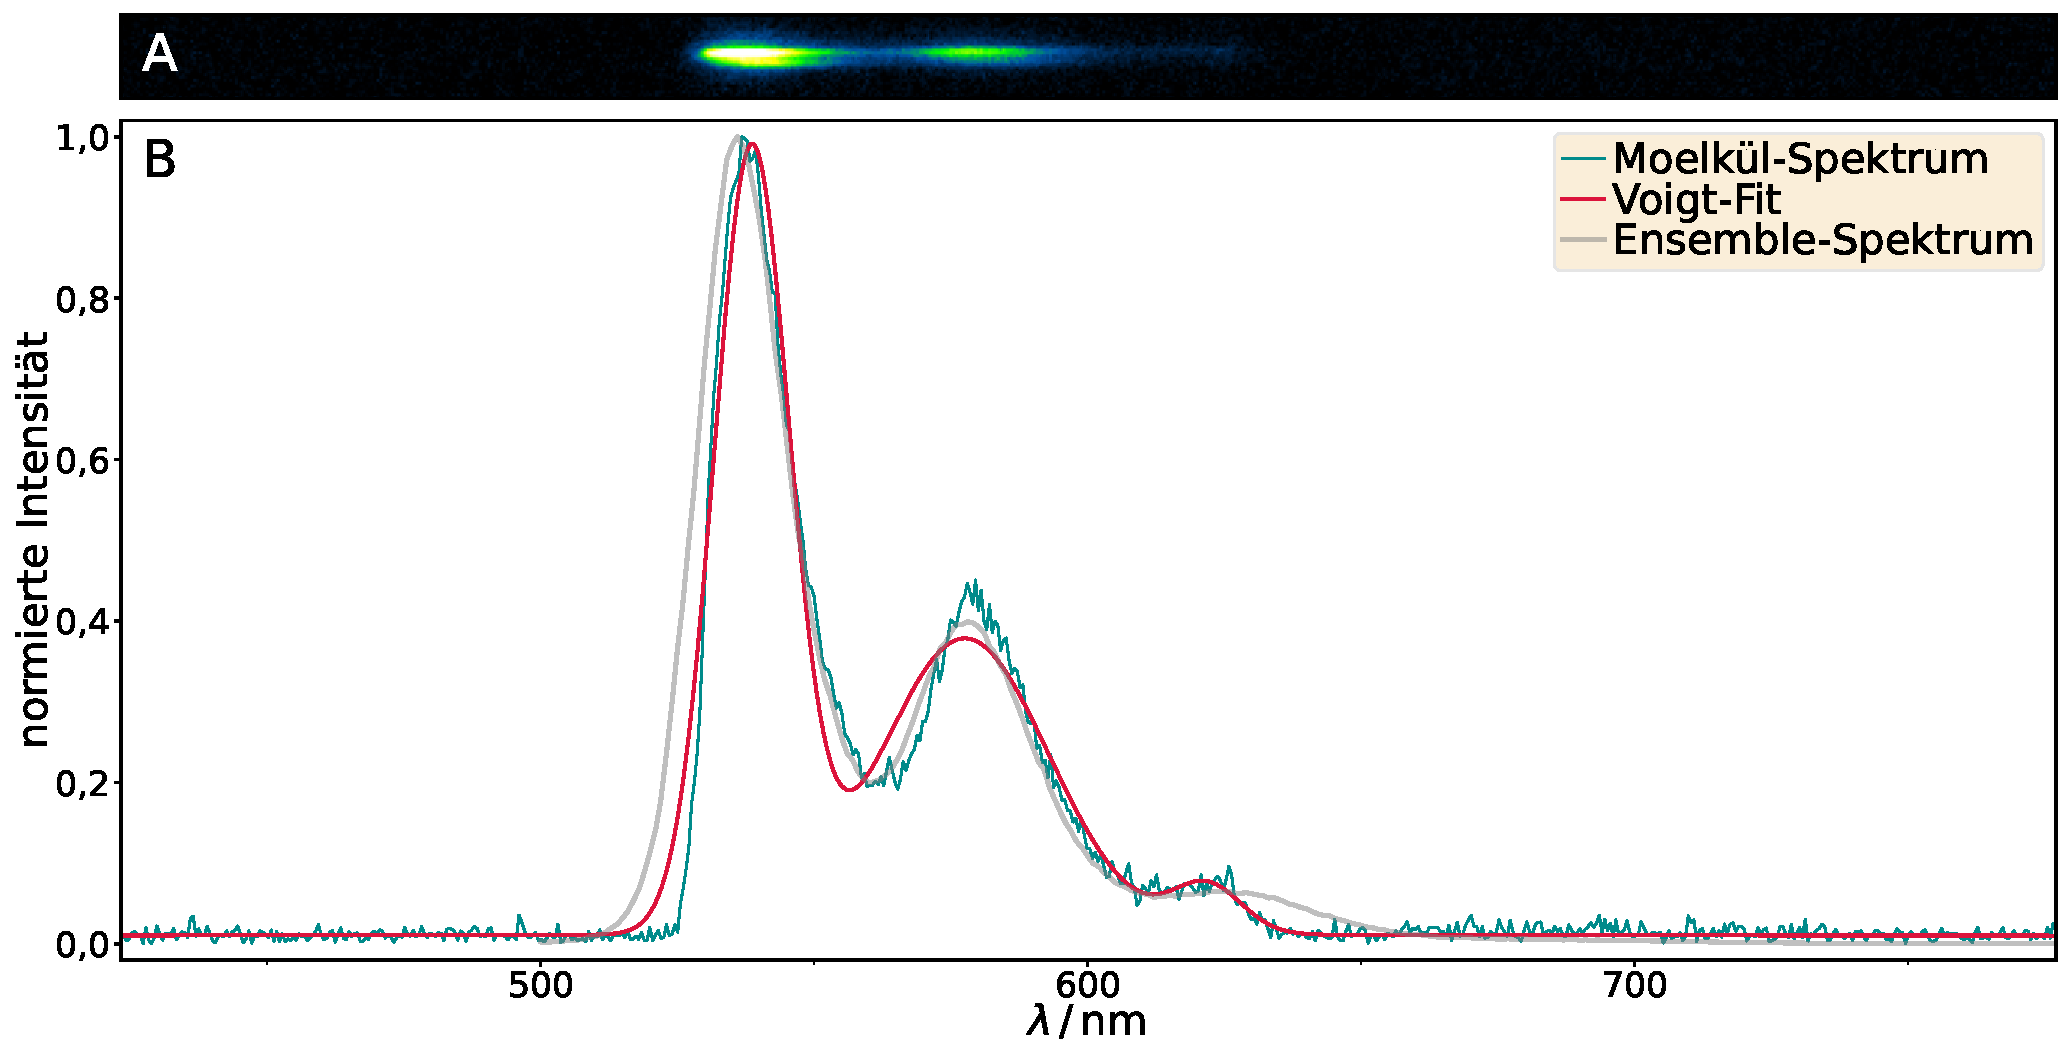
\includegraphics[width=0.49\textwidth]{Spektren/SP10-312.pdf}} \\
    \subfloat[Nummer 19 - $I_{\text{max}}$/a.u.$=142$]{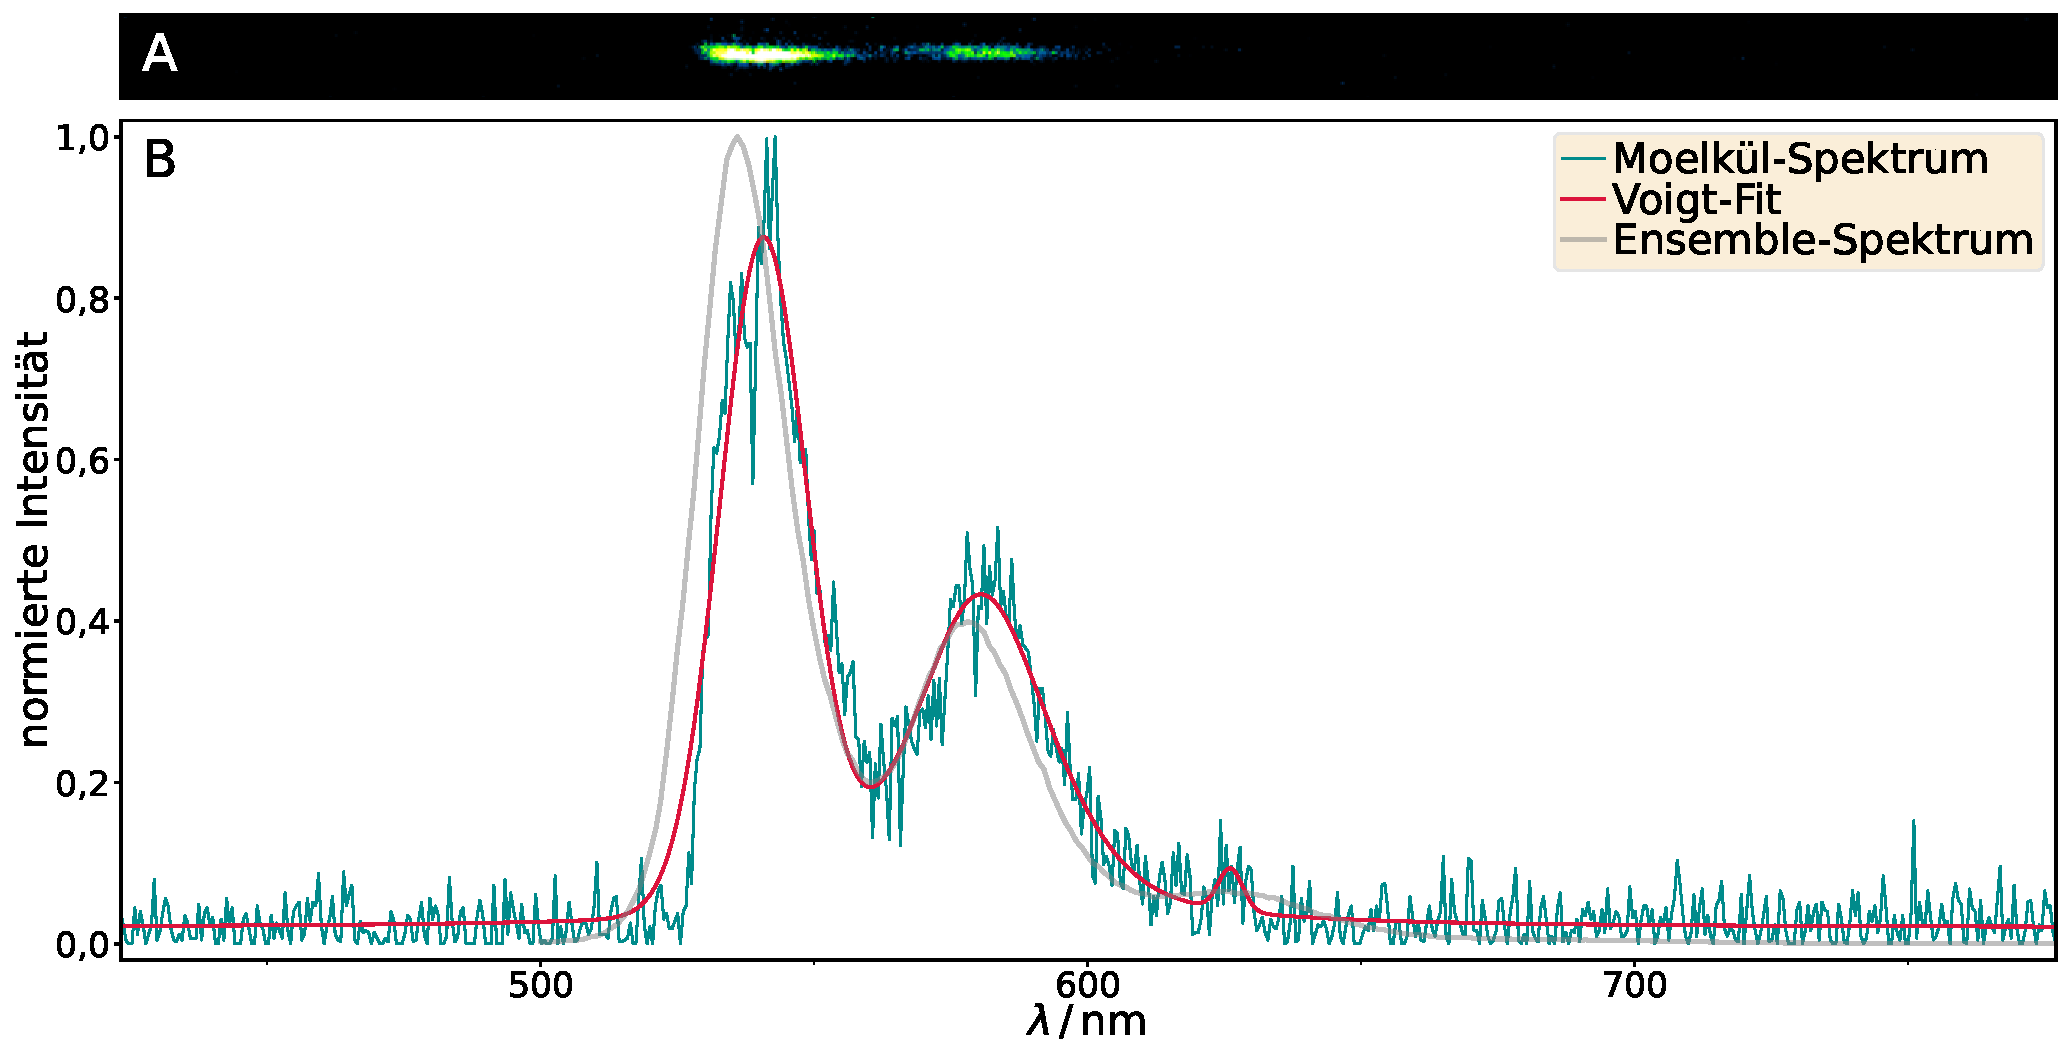
\includegraphics[width=0.49\textwidth]{Spektren/SP19-142.pdf}}
    \subfloat[Nummer 26 - $I_{\text{max}}$/a.u.$=141$]{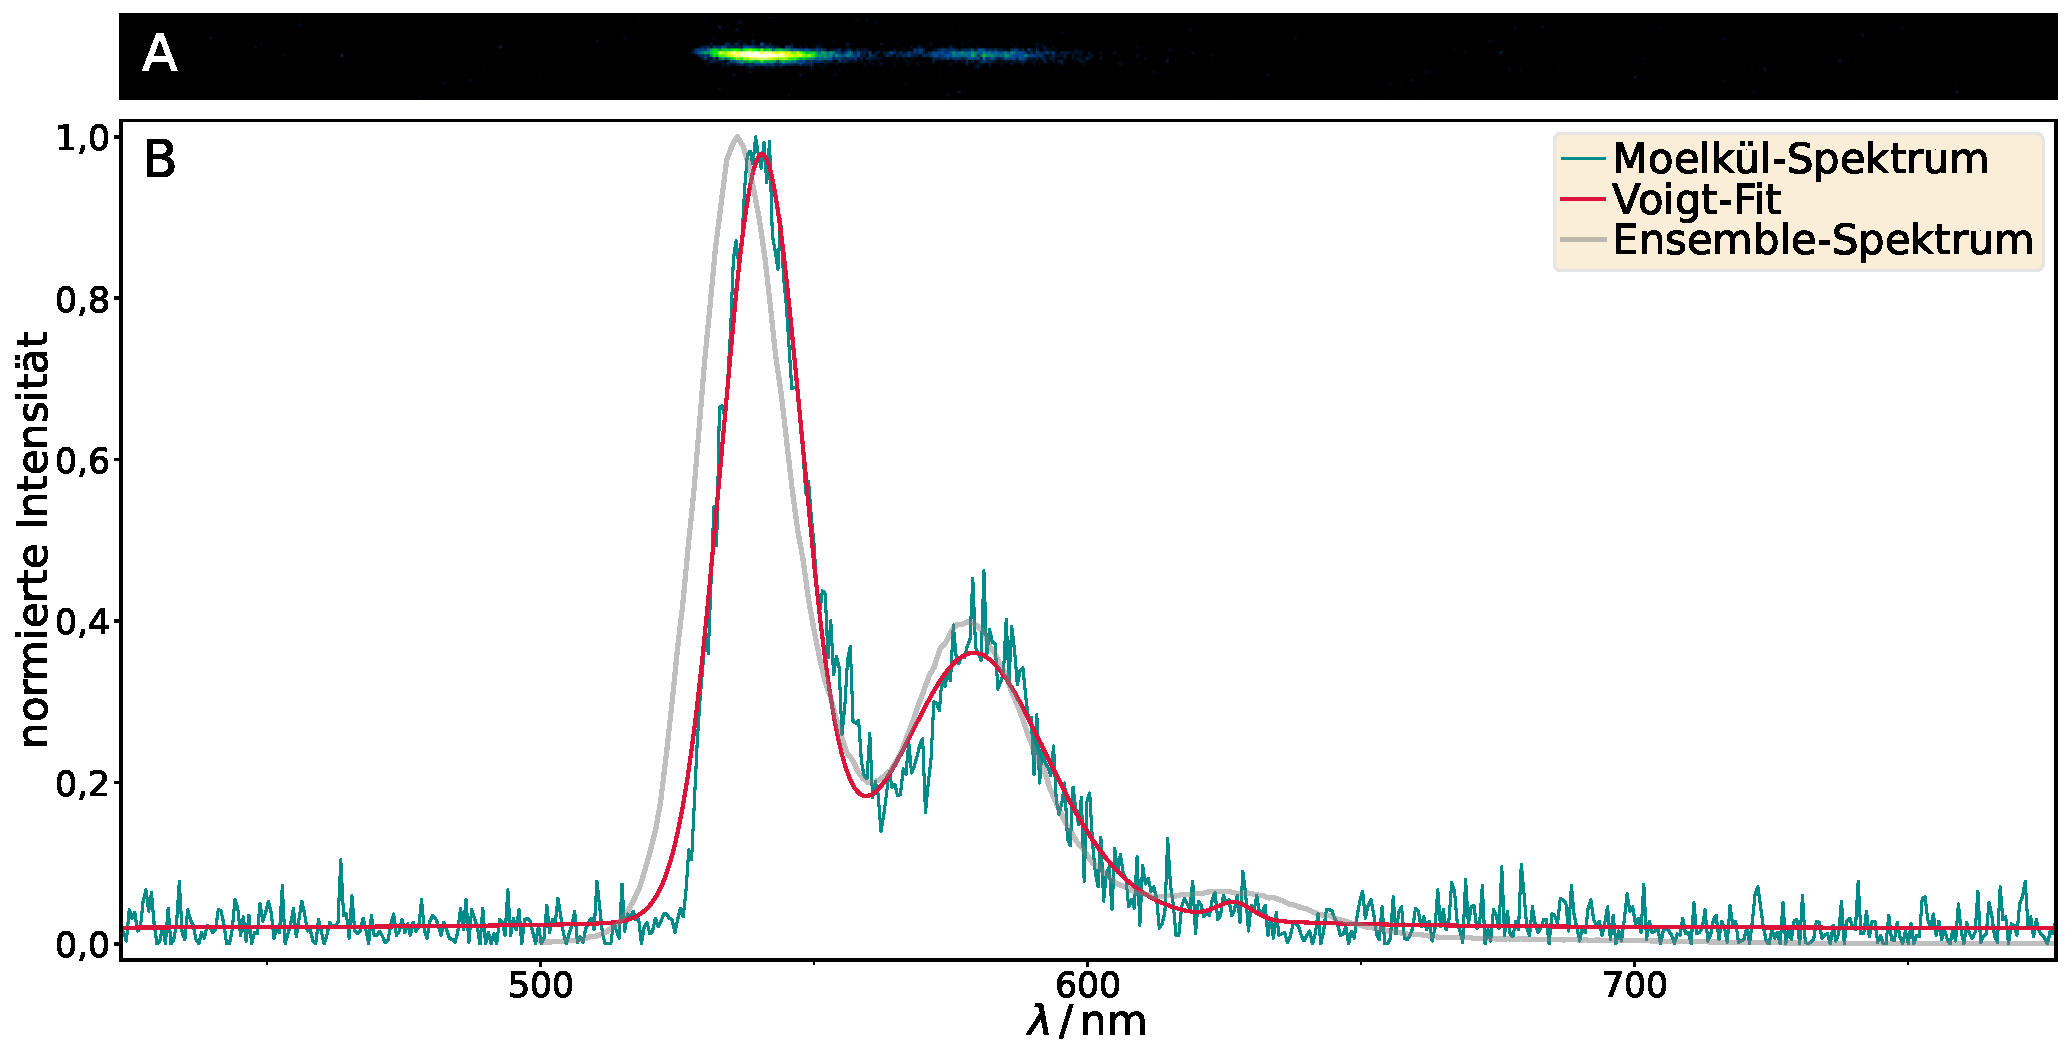
\includegraphics[width=0.49\textwidth]{Spektren/SP26-141.pdf}} 
    \caption{\label{fig:spektren}Vier ausgewählte Einzelmolekülspektren inkl.~dem zugehörigen 
    Pseudo-Voigt-Fit und dem Ensemblespektrum. Es wird jeweils die Nummer des Spektrums angegeben, um 
    einen Vergleich mit Tab.~\ref{tab:lamda} zu erhalten und das in ImageJ bearbeitete Bild des 
    Spektrums (A) angezeigt. Da die Spektren auf die jeweilige Intensitätsspitze normiert sind, 
    ist dieser Wert zusätzlich angegeben.}
\end{figure}  \FloatBarrier
In den ersten beiden Spektren a) und b) ist, aufgrund ihrer hohen Intensität, der 
Übergang $0^{*}\rightarrow2$ deutlich zu erkennen. Die zu den Spektren c) und d) 
gehörigen Moleküle fluoreszieren schwächer, weshalb der betrachtete Übergang im Untergrund 
kaum erkennbar ist. Zusätzlich ist die Linienform der intensiveren Spektren besser definiert.
Die Ergebnisse des Fits für $\lambda_{3}$ sind folglich mit Vorsicht zu betrachten. \\
Abschließen stellen wir die gefitteten Werte der Wellenlängen als Histogramm dar und vergleichen 
dieses mit dem bereitgestellten Ensemblespektrum. Die Ergebnisgrafik ist in Abb.~\ref{fig:histo}
präsentiert.
\begin{figure}[h!]
    \centering
    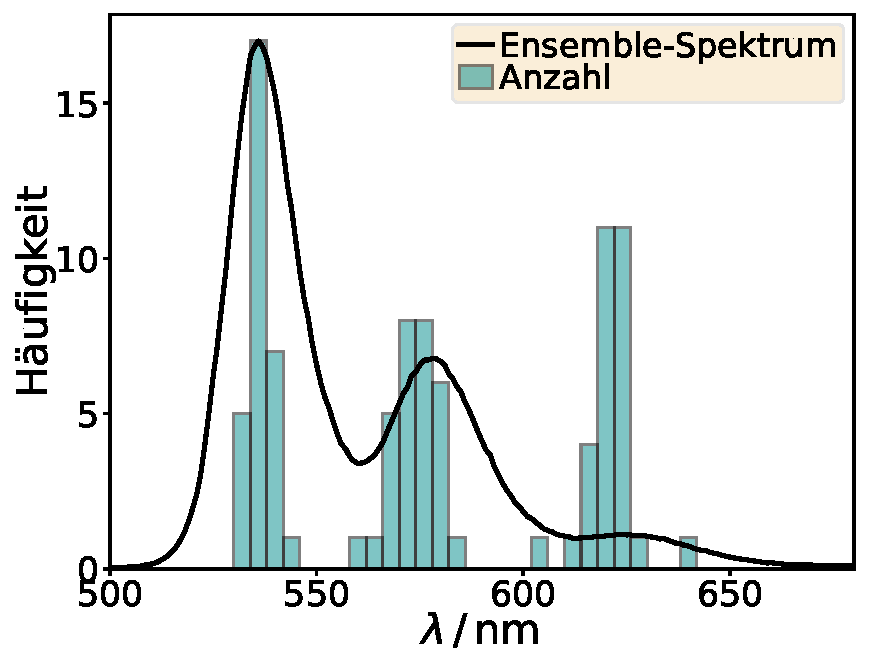
\includegraphics[width=0.6\textwidth]{histo.pdf}
    \caption{\label{fig:histo}Häufigkeit der gefitteten Wellenlängen als Histogramm verglichen mit dem skalierten 
    Ensemblespektrum von PBI.}
\end{figure}\FloatBarrier
Die Bin-Breite des Histogramms wurde am Einzelfehler des Fit-Algorithmuses für die erste Wellenlänge orientiert und auf 
$\Delta{\lambda} = 4\,\si{nm}$ gesetzt. Das Ergebnis sieht jedoch für Breiten bis $\Delta{\lambda} \approx 10\,\si{nm}$
sehr ähnlich aus. 
Zum einen ist $\lambda_{1}$ etwas schärfer als beim Ensemblespektrum definiert. Die Wellenlänge des zweiten Übergangs 
$\lambda_{2}$ scheint bei den Einzelmolekülspektren leicht nach links verschoben zu sein. Die Breite der Verteilung stimmt 
jedoch gut mit dem Ensemblespektrum überein. 
Der letzte Übergang $\lambda_{3}$ erscheint im Histogramm deutlich schärfer definiert als beim Ensemblespektrum. 
Dieser Umstand kann auf den Fit-Algorithmus zurückgeführt werden, der auch eine Wellenlänge errechnet, wenn das Signal im 
Rauschen verschwindet. Dabei ist die Ergebniswellenlänge meist gleich der initialisierten Wellenlänge, die im Bereich 
von $\lambda_{3, \text{initial}} \approx 620\,\si{nm}$ liegt. Insgesamt sieht die Häufigkeitsverteilung ähnlich wie das 
Ensemblespektrum aus, womit die Erwartungen erfüllt sind. Um bessere statistische Aussagen treffen zu können, müsste man 
deutlich mehr Einzelmolekülspektren aufnehmen und sollte bei der Auswahl der Spektren darauf achten, dass der 
Fluoreszenzübergang $0^{*}\rightarrow2$ gut erkennbar ist. \\
Alles in allem sind wir mit den Messergebnissen dieses Versuchsteils sehr zufrieden. Die Einzelmolekülspektren sehen 
gut aus, die Signalstärke liegt im erwarteten oberen Bereich und die Detektierbarkeit während der Versuchsdurchführung 
war zufriedenstellend. \\ 







